% \setchapterpreamble[u]{\margintoc}
\chapter{What I mean by elimination of reflection}
\labch{elim-reflection-intro}

We presented earlier \acrshort{ETT} and its defining reflection rule.
%
\reminder[-1.0cm]{Reflection rule}{
  \begin{equation*}
    \infer[]
      {\xisterm{\Ga}{e}{\Eq{A}{u}{v}}}
      {\xeqterm{\Ga}{u}{v}{A}}
    %
  \end{equation*}
}
%
The next few chapters are going to be dedicated to its elimination from type
theory: that is how to make a translation from \acrshort{ETT} to type theories
that do not feature reflection.

This work gave rise to a publication~\sidecite{winterhalter:hal-01849166} that
focused on translating \acrshort{ETT} to \acrshort{ITT}.
However, with Simon Boulier we worked on another version translating directly to
\acrshort{WTT} which I'm going to present here.

\section{Nature of the translation}

\todo{Have reminders clickable to refer to actual definition.}
\todo{Use the notation table to include the notation of typing etc. especially
the ETT mark.}

\subsection{Syntactical translations are not possible}

First of all we have to wonder about what kind of translation is possible.
We presented earlier~\misref{} the notion of syntactical translation.
Unfortunately it is not possible to devise a syntactical translation to
eliminate reflection from type theory.

Assume we have such a translation given by \(\transl{.}\) and \([.]\) such that
whenever \(\xisterm{\Gamma}{t}{A}\) we have
\(\isterm{\transl{\Gamma}}{[t]}{\transl{A}}\) in the target type theory.
Now let's say we have an inconsistent context in \acrshort{ETT}: \(\Gamma_\bot\)
(one can for instance assume \(0 = 1\) or \(\forall A, A\)), in such a context
anything can have any type because conversion has become trivial.
%
\marginnote[1.4cm]{
  Since \(\Gamma_\bot\) is inconsistent, anything can be proved from it,
  including the equality between the two types \(\mathbb{N}\) and \(\bot\).
  We then use reflection and conversion.
}
\begin{mathpar}
  \infer
    {
      \infer
        {\vdots}
        {\xisterm{\Gamma_\bot}{0}{\mathbb{N}}}
      \\
      \infer
        {
          \infer
            {\vdots}
            {\xisterm{\Gamma_\bot}{\_}{\mathbb{N} = \bot}}
          %
        }
        {\xeqterm{\Gamma_\bot}{\mathbb{N}}{\bot}{\Type}}
    }
    {\xisterm{\Gamma_\bot}{0}{\bot}}
  %
\end{mathpar}
%
It thus follows that in the target you have
\( \isterm{\transl{\Gamma_\bot}}{[0]}{\transl{\bot}} \).
Similarly you would have
\( \isterm{\transl{\Gamma_\bot}}{[0]}{\transl{\mathbb{N}}} \). This means
that both \(\bot\) and \(\mathbb{N}\) should be translated to similar things
(to convertible types in case the target theory has uniqueness of type), without
being able to exploit the knowledge that \(\Gamma_\bot\) is inconsistent
because of the syntactical nature of the translation.

\todo{Make things clearer}
Even worse, translations should preserve falsehood meaning in particular that
the translation of \(0\) should imply a proof of \(\bot\) in the target.
This is not a concrete proof that it is impossible but rather an argument
to see that such a translation would not behave well. One of the reasons is
that it would translate terms, types and contexts independently when it cannot.
Another is that an \acrshort{ETT} term does not contain any hints with respect
to the uses of reflection.

\subsection{Our translation(s)}

If we go back to the notion of proof~\misref, it becomes apparent that
syntactical translations do not work because we would not be translating proofs
but only partial ones; in other words terms in \acrshort{ETT} are not proofs
because they are insufficient to recover a typing derivation\sidenote{Because
type-checking is undecidable.}.
Thus comes the question of what is a \emph{suitable proof} in \acrshort{ETT}.
There is probably an intermediate structure between the term and the full
derivation that fits this role in the form of a term together with explicit
casts, however, in the setting of this thesis, we will still use complete
typing derivations in \acrshort{ETT} as \emph{proofs}.

Many problems stem from this approach unfortunately. Since we're translating
derivations there is no guarantee that the same term \(t\) in
\(\xisterm{\Gamma}{t}{A}\) and \(\xisterm{\Delta}{t}{B}\) will be translated
twice to the same term, this actually goes even for two different derivations
of the same judgement \(\xisterm{\Gamma}{t}{A}\).
This seems like a big obstacle to compositionality and would be iredeemable
without extra care regarding how individual judgements are translated.

We solve these problems by relating translations of a term (respectively
type and context) to the term itself, \emph{syntactically}.

\section{Target(s) of the translation}

Strictly speaking, elimination of reflection should be a translation from a
certain type theory \(T\) extended with reflection to \(T\) itself.
To fit this framework, we would provide a translation from \acrshort{ETT}
to \acrshort{ITT}. With Simon Boulier we discovered however that it is possible
to do something even stronger and go directly to a much weaker theory where
the notion of conversion is removed, \acrshort{WTT}.

\begin{figure}[hb]
  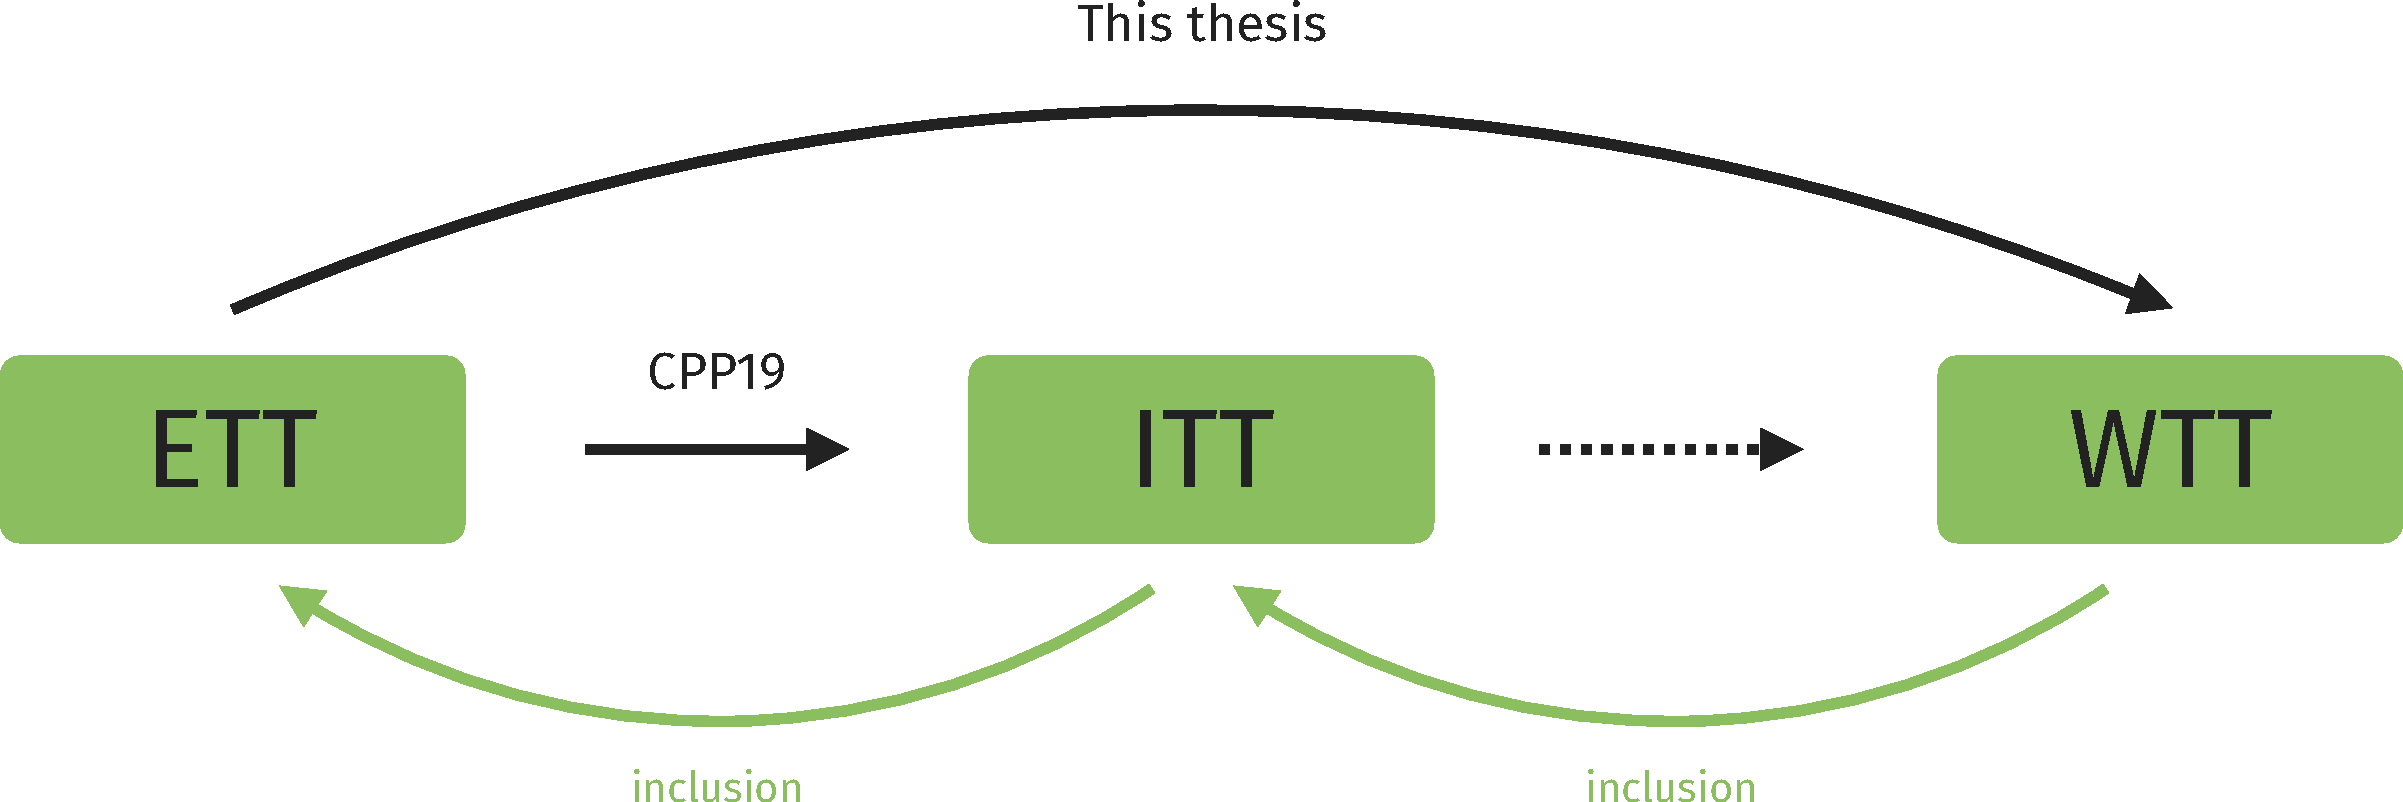
\includegraphics[width=0.9\textwidth]{images/elim-reflection-summary}
\end{figure}

From a translation of \acrshort{ETT} to \acrshort{WTT} we get an indirect one
from \acrshort{ETT} to \acrshort{ITT} as well as one from \acrshort{ITT} to
\acrshort{WTT}.
\marginnote[-0.5cm]{In both cases we exploit the fact that \acrshort{ETT} extends
\acrshort{ITT} which in turn extends \acrshort{WTT}.}

\section{Goal of the translation}

\todo{Motivations should come first, but it's hard to do it without saying
what we're motivating...}

\todo{Consistency of course, but mainly conservativity, and why not some
practical uses in the future? Probably after coming up with a proper notion
of proof in ETT.}
\todo{Talk about what it teaches us with respect to computation}

Why would we want to eliminate reflection?